\section{Calibration from Real Charging Data}
\label{sec:calibration}

The behavioral layer is calibrated per region from real charging corpora. The
pipeline is: normalize a source corpus; summarize each real driver by the
axes $(\phifreq, \kapcons, \deldist)$; assign drivers to regions; fit each
region's distributions by maximum likelihood; and write the fitted parameters,
sample sizes, fit quality, and provenance back into the population library
that generation consumes.

\subsection{Sources}
\label{sec:sources}

Table~\ref{tab:sources} summarizes the corpora. Each source has its own
normalizer and its own region geometry: region boxes are anchored on each
corpus's empirical $(\phifreq,\kapcons)$ cloud rather than shared, so one
dataset's assumptions are not imposed on another. For ElaadNL this
re-anchoring reduced unassigned drivers from 76\% to 0\%; the ACN grid
predates the exercise and its re-anchoring is noted as future work
(\S\ref{sec:limitations}). The INL EV Project cohort is included as a
\emph{fixture-calibrated} legacy population: its parameters are hand-seeded to
the published fleet character (24\,kWh-era vehicles) rather than fitted from
raw records, and it is released---so labeled---as a distribution-shift
benchmark rather than claimed as a calibration corpus.

\begin{table}[t]
\caption{Calibration sources. ``Fitted'' populations carry per-region MLE
parameters with recorded provenance; the INL cohort is a labeled fixture.
\owed{Regenerate counts with WS-F; EV WATTS row from populations.yaml
metadata.}}
\label{tab:sources}
\centering\small
\begin{tabular}{@{}lllll@{}}
\toprule
Corpus & Span & Venue & Scale & Policy \\
\midrule
ACN-Data & 2019--21 & workplace (3 sites) & 632 users / 41{,}774 sessions & fitted \\
EV~WATTS & 2019--23 & workplace (public rel.) & 1{,}265{,}017 sessions & fitted \\
ElaadNL & 2020--24 & EU public & 55{,}379 sessions / 1{,}231 drivers & fitted \\
INL EVP & 2011--13 & residential & fixture (65 sessions) & fixture \\
\bottomrule
\end{tabular}
\end{table}

\subsection{Axes, regions, and assignment}

For each real driver we compute $\phifreq$ (share of active days with a
session), $\kapcons$ (timing consistency of arrivals), and $\deldist$ (a
distance proxy). Drivers fall into the first region box containing their
$(\phifreq,\kapcons)$; unassigned fractions are 0--0.5\% on the current grids.
Region \emph{weights} are the empirical user shares---for ACN:
rare-consistent 36.1\%, occasional-consistent 39.8\%, regular-charger 23.0\%,
rare-inconsistent 0.6\%---so the generated population reproduces the observed
cohort composition, not a designer's guess. The empirical geometry is itself
informative (Fig.~\ref{fig:axes}): real workplace drivers plug in far less
often than intuition suggests (76\% of ACN drivers at $\phifreq \le 0.3$),
which the calibrated grids encode and hand-authored grids would have missed.

\begin{figure}[t]
  \centering
  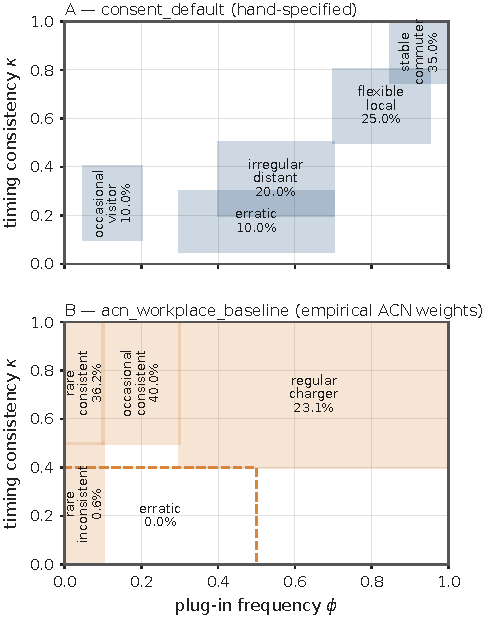
\includegraphics[width=\linewidth]{figures/fig2_axes.pdf}
  \caption{Region geometries in the $(\phifreq,\kapcons)$ plane. Top: the
  hand-specified \texttt{consent\_default} grid concentrates mass at high
  plug-in frequency. Bottom: the ACN-anchored grid, with empirical user-share
  weights, places 76\% of drivers at $\phifreq \le 0.3$; the dashed box is a
  region with zero empirical weight.}
  \label{fig:axes}
\end{figure}

\subsection{Per-region distribution fitting}

Within each region we fit: arrival hour by truncated-normal maximum likelihood
on a $[4,22]$\,h window, upgraded to a $k$-component mixture only when the
mixture improves the Kolmogorov--Smirnov distance by at least $0.02$; dwell by
Weibull MLE with the same mixture rule; and the arrival--dwell dependence by a
Gaussian copula with $\rho$ obtained from the Spearman rank correlation.
Mixture fits require at least 60 sessions and any fit at least 30; smaller
cells fall back to pooled fits. Fitting is per region rather than pooled: the
largest ACN region (rare-consistent, 36\% of drivers) arrives systematically
later than the pooled corpus, and replacing a broadcast pooled fit with its
own fit reduced its arrival KS from $0.179$ to $0.079$. The fitted arrival
distribution for that region is bimodal (morning and early-afternoon
components), a structure a single truncated normal cannot express
(Fig.~\ref{fig:arrival}).

\begin{figure}[t]
  \centering
  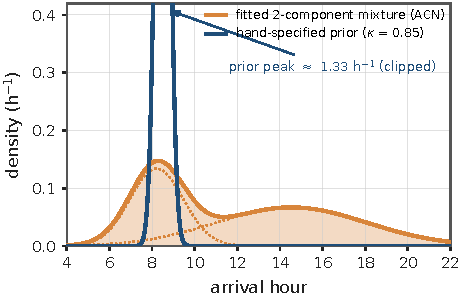
\includegraphics[width=\linewidth]{figures/fig3_arrival.pdf}
  \caption{Arrival-hour density for the largest ACN region: hand-specified
  prior (unimodal truncated normal) versus the fitted two-component mixture
  ($0.42\,\mathcal{N}(8.21, 1.25) + 0.58\,\mathcal{N}(14.54, 3.52)$, truncated
  to $[4,22]$\,h). Real workplace arrivals are bimodal.}
  \label{fig:arrival}
\end{figure}

\subsection{The SoC contract}
\label{sec:soc}

No public charging dataset records state of charge: equipment meters energy.
Both SoC channels are therefore \emph{modeled priors made consistent with
observed energy}, and we state the reconstruction explicitly. Arrival SoC is
drawn from a shared, seeded prior; the required departure SoC is calibrated
per region as the arrival prior plus delivered energy over inferred battery
capacity---delivered energy being the one universally recorded real signal.
Battery capacity is inferred per driver from maximum observed session energy,
falling back to vehicle-class defaults for roughly a third of ACN drivers.
Every SoC-related fitted value carries a provenance stamp identifying this
contract, and the datasheet repeats it. We regard the explicitness of this
contract as a feature of the release: downstream users can accept, replace,
or stress the prior, but cannot mistake it for measurement.
